\documentclass{standalone}
\usepackage{tikz}
\usetikzlibrary{patterns, positioning}

\begin{document}
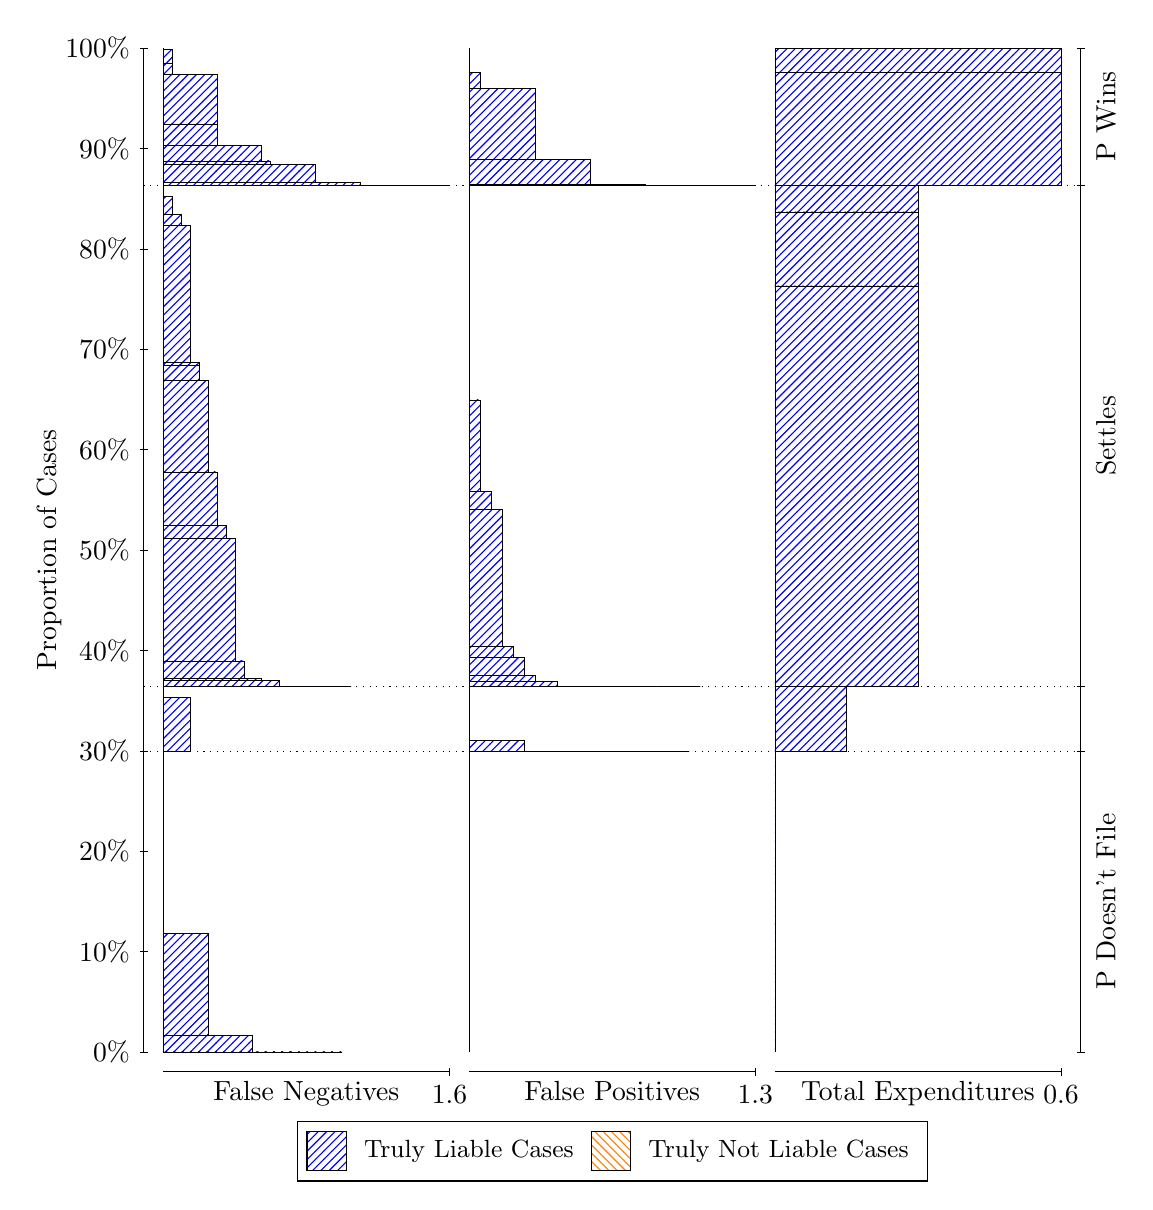
\begin{tikzpicture}
\draw[black, very thin] (1.5,1.75) -- (1.5,14.5);
\node[rotate=90, anchor=center] at (0.3, 8.125) {Proportion of Cases};
\draw[black, very thin] (1.45,1.75) -- (1.55,1.75);
\node[anchor=east] at (1.45, 1.75) {0\%};
\draw[black, very thin] (1.45,3.025) -- (1.55,3.025);
\node[anchor=east] at (1.45, 3.025) {10\%};
\draw[black, very thin] (1.45,4.3) -- (1.55,4.3);
\node[anchor=east] at (1.45, 4.3) {20\%};
\draw[black, very thin] (1.45,5.575) -- (1.55,5.575);
\node[anchor=east] at (1.45, 5.575) {30\%};
\draw[black, very thin] (1.45,6.85) -- (1.55,6.85);
\node[anchor=east] at (1.45, 6.85) {40\%};
\draw[black, very thin] (1.45,8.125) -- (1.55,8.125);
\node[anchor=east] at (1.45, 8.125) {50\%};
\draw[black, very thin] (1.45,9.4) -- (1.55,9.4);
\node[anchor=east] at (1.45, 9.4) {60\%};
\draw[black, very thin] (1.45,10.675) -- (1.55,10.675);
\node[anchor=east] at (1.45, 10.675) {70\%};
\draw[black, very thin] (1.45,11.95) -- (1.55,11.95);
\node[anchor=east] at (1.45, 11.95) {80\%};
\draw[black, very thin] (1.45,13.225) -- (1.55,13.225);
\node[anchor=east] at (1.45, 13.225) {90\%};
\draw[black, very thin] (1.45,14.5) -- (1.55,14.5);
\node[anchor=east] at (1.45, 14.5) {100\%};

\draw[black, very thin] (13.4,1.75) -- (13.4,14.5);
\draw[black, very thin] (13.35,1.75) -- (13.45,1.75);
\node[anchor=west] at (13.35, 1.75) {};
\draw[black, very thin] (13.35,5.5706) -- (13.45,5.5706);
\node[anchor=west] at (13.35, 5.5706) {};
\draw[black, very thin] (13.35,6.3924) -- (13.45,6.3924);
\node[anchor=west] at (13.35, 6.3924) {};
\draw[black, very thin] (13.35,12.755) -- (13.45,12.755);
\node[anchor=west] at (13.35, 12.755) {};
\draw[black, very thin] (13.35,14.5) -- (13.45,14.5);
\node[anchor=west] at (13.35, 14.5) {};

\draw[black, very thin, pattern color=blue, pattern=north east lines] (1.75,1.75) rectangle (4.0208,1.75);
\draw[black, very thin, pattern color=blue, pattern=north east lines] (1.75,1.75) rectangle (3.4531,1.7518);
\draw[black, very thin, pattern color=blue, pattern=north east lines] (1.75,1.7518) rectangle (2.8854,1.961);
\draw[black, very thin, pattern color=blue, pattern=north east lines] (1.75,1.961) rectangle (2.3177,3.2569);
\draw[black, very thin, pattern color=orange, pattern=north west lines] (1.75,3.2569) rectangle (1.75,3.2569);
\draw[black, very thin, pattern color=blue, pattern=north east lines] (1.75,3.2569) rectangle (1.75,5.5706);
\draw[black, very thin, pattern color=blue, pattern=north east lines] (1.75,5.5706) rectangle (2.0906,6.258);
\draw[black, very thin, pattern color=orange, pattern=north west lines] (1.75,6.258) rectangle (1.75,6.258);
\draw[black, very thin, pattern color=blue, pattern=north east lines] (1.75,6.258) rectangle (1.75,6.3924);
\draw[black, very thin, pattern color=blue, pattern=north east lines] (1.75,6.3924) rectangle (4.1344,6.3924);
\draw[black, very thin, pattern color=blue, pattern=north east lines] (1.75,6.3924) rectangle (3.9073,6.3924);
\draw[black, very thin, pattern color=blue, pattern=north east lines] (1.75,6.3924) rectangle (3.6802,6.3924);
\draw[black, very thin, pattern color=blue, pattern=north east lines] (1.75,6.3924) rectangle (3.5667,6.3924);
\draw[black, very thin, pattern color=blue, pattern=north east lines] (1.75,6.3924) rectangle (3.3396,6.3924);
\draw[black, very thin, pattern color=blue, pattern=north east lines] (1.75,6.3924) rectangle (3.226,6.4677);
\draw[black, very thin, pattern color=blue, pattern=north east lines] (1.75,6.4677) rectangle (3.1125,6.4691);
\draw[black, very thin, pattern color=blue, pattern=north east lines] (1.75,6.4691) rectangle (2.999,6.4985);
\draw[black, very thin, pattern color=blue, pattern=north east lines] (1.75,6.4985) rectangle (2.7719,6.7147);
\draw[black, very thin, pattern color=blue, pattern=north east lines] (1.75,6.7147) rectangle (2.7719,6.7163);
\draw[black, very thin, pattern color=blue, pattern=north east lines] (1.75,6.7163) rectangle (2.6583,8.269);
\draw[black, very thin, pattern color=blue, pattern=north east lines] (1.75,8.269) rectangle (2.5448,8.4331);
\draw[black, very thin, pattern color=blue, pattern=north east lines] (1.75,8.4331) rectangle (2.4312,9.1166);
\draw[black, very thin, pattern color=blue, pattern=north east lines] (1.75,9.1166) rectangle (2.3177,10.282);
\draw[black, very thin, pattern color=blue, pattern=north east lines] (1.75,10.282) rectangle (2.2042,10.476);
\draw[black, very thin, pattern color=blue, pattern=north east lines] (1.75,10.476) rectangle (2.2042,10.507);
\draw[black, very thin, pattern color=blue, pattern=north east lines] (1.75,10.507) rectangle (2.0906,12.248);
\draw[black, very thin, pattern color=blue, pattern=north east lines] (1.75,12.248) rectangle (1.9771,12.383);
\draw[black, very thin, pattern color=blue, pattern=north east lines] (1.75,12.383) rectangle (1.8635,12.613);
\draw[black, very thin, pattern color=orange, pattern=north west lines] (1.75,12.613) rectangle (1.75,12.613);
\draw[black, very thin, pattern color=blue, pattern=north east lines] (1.75,12.613) rectangle (1.75,12.755);
\draw[black, very thin, pattern color=blue, pattern=north east lines] (1.75,12.755) rectangle (5.3833,12.755);
\draw[black, very thin, pattern color=blue, pattern=north east lines] (1.75,12.755) rectangle (4.8156,12.756);
\draw[black, very thin, pattern color=blue, pattern=north east lines] (1.75,12.756) rectangle (4.2479,12.791);
\draw[black, very thin, pattern color=blue, pattern=north east lines] (1.75,12.791) rectangle (4.1344,12.791);
\draw[black, very thin, pattern color=blue, pattern=north east lines] (1.75,12.791) rectangle (3.6802,13.027);
\draw[black, very thin, pattern color=blue, pattern=north east lines] (1.75,13.027) rectangle (3.5667,13.027);
\draw[black, very thin, pattern color=blue, pattern=north east lines] (1.75,13.027) rectangle (3.1125,13.068);
\draw[black, very thin, pattern color=blue, pattern=north east lines] (1.75,13.068) rectangle (2.999,13.267);
\draw[black, very thin, pattern color=blue, pattern=north east lines] (1.75,13.267) rectangle (2.5448,13.267);
\draw[black, very thin, pattern color=blue, pattern=north east lines] (1.75,13.267) rectangle (2.4312,13.536);
\draw[black, very thin, pattern color=blue, pattern=north east lines] (1.75,13.536) rectangle (2.4312,14.17);
\draw[black, very thin, pattern color=blue, pattern=north east lines] (1.75,14.17) rectangle (1.9771,14.17);
\draw[black, very thin, pattern color=blue, pattern=north east lines] (1.75,14.17) rectangle (1.8635,14.309);
\draw[black, very thin, pattern color=blue, pattern=north east lines] (1.75,14.309) rectangle (1.8635,14.483);
\draw[black, very thin, pattern color=orange, pattern=north west lines] (1.75,14.483) rectangle (1.75,14.483);
\draw[black, very thin, pattern color=blue, pattern=north east lines] (1.75,14.483) rectangle (1.75,14.5);
\draw[black, very thin, pattern color=orange, pattern=north west lines] (5.6333,1.75) rectangle (5.6333,1.75);
\draw[black, very thin, pattern color=blue, pattern=north east lines] (5.6333,1.75) rectangle (5.6333,5.5706);
\draw[black, very thin, pattern color=orange, pattern=north west lines] (5.6333,5.5706) rectangle (8.4282,5.5706);
\draw[black, very thin, pattern color=blue, pattern=north east lines] (5.6333,5.5706) rectangle (8.4282,5.5706);
\draw[black, very thin, pattern color=blue, pattern=north east lines] (5.6333,5.5706) rectangle (7.7295,5.5706);
\draw[black, very thin, pattern color=blue, pattern=north east lines] (5.6333,5.5706) rectangle (7.0308,5.5716);
\draw[black, very thin, pattern color=blue, pattern=north east lines] (5.6333,5.5716) rectangle (6.3321,5.705);
\draw[black, very thin, pattern color=blue, pattern=north east lines] (5.6333,5.705) rectangle (5.6333,6.3924);
\draw[black, very thin, pattern color=orange, pattern=north west lines] (5.6333,6.3924) rectangle (8.5679,6.3924);
\draw[black, very thin, pattern color=blue, pattern=north east lines] (5.6333,6.3924) rectangle (8.5679,6.3924);
\draw[black, very thin, pattern color=orange, pattern=north west lines] (5.6333,6.3924) rectangle (8.009,6.3924);
\draw[black, very thin, pattern color=blue, pattern=north east lines] (5.6333,6.3924) rectangle (8.009,6.3924);
\draw[black, very thin, pattern color=blue, pattern=north east lines] (5.6333,6.3924) rectangle (7.8692,6.3924);
\draw[black, very thin, pattern color=orange, pattern=north west lines] (5.6333,6.3924) rectangle (7.45,6.3924);
\draw[black, very thin, pattern color=blue, pattern=north east lines] (5.6333,6.3924) rectangle (7.45,6.3924);
\draw[black, very thin, pattern color=blue, pattern=north east lines] (5.6333,6.3924) rectangle (7.3103,6.3924);
\draw[black, very thin, pattern color=blue, pattern=north east lines] (5.6333,6.3924) rectangle (7.1705,6.3925);
\draw[black, very thin, pattern color=orange, pattern=north west lines] (5.6333,6.3925) rectangle (6.891,6.3925);
\draw[black, very thin, pattern color=blue, pattern=north east lines] (5.6333,6.3925) rectangle (6.891,6.3929);
\draw[black, very thin, pattern color=blue, pattern=north east lines] (5.6333,6.3929) rectangle (6.7513,6.4571);
\draw[black, very thin, pattern color=orange, pattern=north west lines] (5.6333,6.4571) rectangle (6.6115,6.4571);
\draw[black, very thin, pattern color=blue, pattern=north east lines] (5.6333,6.4571) rectangle (6.6115,6.4613);
\draw[black, very thin, pattern color=blue, pattern=north east lines] (5.6333,6.4613) rectangle (6.4718,6.535);
\draw[black, very thin, pattern color=orange, pattern=north west lines] (5.6333,6.535) rectangle (6.3321,6.535);
\draw[black, very thin, pattern color=blue, pattern=north east lines] (5.6333,6.535) rectangle (6.3321,6.7646);
\draw[black, very thin, pattern color=blue, pattern=north east lines] (5.6333,6.7646) rectangle (6.1923,6.8994);
\draw[black, very thin, pattern color=blue, pattern=north east lines] (5.6333,6.8994) rectangle (6.0526,8.6411);
\draw[black, very thin, pattern color=blue, pattern=north east lines] (5.6333,8.6411) rectangle (5.9128,8.8659);
\draw[black, very thin, pattern color=blue, pattern=north east lines] (5.6333,8.8659) rectangle (5.7731,10.031);
\draw[black, very thin, pattern color=blue, pattern=north east lines] (5.6333,10.031) rectangle (5.6333,12.755);
\draw[black, very thin, pattern color=orange, pattern=north west lines] (5.6333,12.755) rectangle (9.2667,12.755);
\draw[black, very thin, pattern color=blue, pattern=north east lines] (5.6333,12.755) rectangle (9.2667,12.755);
\draw[black, very thin, pattern color=orange, pattern=north west lines] (5.6333,12.755) rectangle (8.5679,12.755);
\draw[black, very thin, pattern color=blue, pattern=north east lines] (5.6333,12.755) rectangle (8.5679,12.756);
\draw[black, very thin, pattern color=orange, pattern=north west lines] (5.6333,12.756) rectangle (7.8692,12.756);
\draw[black, very thin, pattern color=blue, pattern=north east lines] (5.6333,12.756) rectangle (7.8692,12.773);
\draw[black, very thin, pattern color=orange, pattern=north west lines] (5.6333,12.773) rectangle (7.1705,12.773);
\draw[black, very thin, pattern color=blue, pattern=north east lines] (5.6333,12.773) rectangle (7.1705,13.085);
\draw[black, very thin, pattern color=orange, pattern=north west lines] (5.6333,13.085) rectangle (7.0308,13.085);
\draw[black, very thin, pattern color=blue, pattern=north east lines] (5.6333,13.085) rectangle (7.0308,13.085);
\draw[black, very thin, pattern color=blue, pattern=north east lines] (5.6333,13.085) rectangle (6.4718,13.988);
\draw[black, very thin, pattern color=orange, pattern=north west lines] (5.6333,13.988) rectangle (6.3321,13.988);
\draw[black, very thin, pattern color=blue, pattern=north east lines] (5.6333,13.988) rectangle (6.3321,13.988);
\draw[black, very thin, pattern color=blue, pattern=north east lines] (5.6333,13.988) rectangle (5.7731,14.188);
\draw[black, very thin, pattern color=orange, pattern=north west lines] (5.6333,14.188) rectangle (5.6333,14.188);
\draw[black, very thin, pattern color=blue, pattern=north east lines] (5.6333,14.188) rectangle (5.6333,14.5);
\draw[black, very thin, pattern color=orange, pattern=north west lines] (9.5167,1.75) rectangle (9.5167,1.75);
\draw[black, very thin, pattern color=blue, pattern=north east lines] (9.5167,1.75) rectangle (9.5167,5.5706);
\draw[black, very thin, pattern color=orange, pattern=north west lines] (9.5167,5.5706) rectangle (10.425,5.5706);
\draw[black, very thin, pattern color=blue, pattern=north east lines] (9.5167,5.5706) rectangle (10.425,6.3924);
\draw[black, very thin, pattern color=orange, pattern=north west lines] (9.5167,6.3924) rectangle (11.333,6.3924);
\draw[black, very thin, pattern color=blue, pattern=north east lines] (9.5167,6.3924) rectangle (11.333,11.478);
\draw[black, very thin, pattern color=orange, pattern=north west lines] (9.5167,11.478) rectangle (11.333,11.478);
\draw[black, very thin, pattern color=blue, pattern=north east lines] (9.5167,11.478) rectangle (11.333,12.42);
\draw[black, very thin, pattern color=orange, pattern=north west lines] (9.5167,12.42) rectangle (11.333,12.42);
\draw[black, very thin, pattern color=blue, pattern=north east lines] (9.5167,12.42) rectangle (11.333,12.755);
\draw[black, very thin, pattern color=orange, pattern=north west lines] (9.5167,12.755) rectangle (13.15,12.755);
\draw[black, very thin, pattern color=blue, pattern=north east lines] (9.5167,12.755) rectangle (13.15,14.188);
\draw[black, very thin, pattern color=orange, pattern=north west lines] (9.5167,14.188) rectangle (13.15,14.188);
\draw[black, very thin, pattern color=blue, pattern=north east lines] (9.5167,14.188) rectangle (13.15,14.5);
\draw[black, dotted] (1.5,5.5706) -- (13.4,5.5706);
\draw[black, dotted] (1.5,6.3924) -- (13.4,6.3924);
\draw[black, dotted] (1.5,12.755) -- (13.4,12.755);
\draw[black, very thin] (1.75,1.5) -- (5.3833,1.5);
\node[anchor=north] at (3.5667, 1.5) {False Negatives};
\draw[black, very thin] (5.3833,1.45) -- (5.3833,1.55);
\node[anchor=north] at (5.3833, 1.45) {1.6};

\draw[black, very thin] (5.6333,1.5) -- (9.2667,1.5);
\node[anchor=north] at (7.45, 1.5) {False Positives};
\draw[black, very thin] (9.2667,1.45) -- (9.2667,1.55);
\node[anchor=north] at (9.2667, 1.45) {1.3};

\draw[black, very thin] (9.5167,1.5) -- (13.15,1.5);
\node[anchor=north] at (11.333, 1.5) {Total Expenditures};
\draw[black, very thin] (13.15,1.45) -- (13.15,1.55);
\node[anchor=north] at (13.15, 1.45) {0.6};

\node[black, centered, rotate=90] at (13.72, 3.6603) {P Doesn't File};

\node[black, centered, rotate=90] at (13.72, 9.574) {Settles};
\node[black, centered, rotate=90] at (13.72, 13.628) {P Wins};

\draw (7.449999999999999,1.5) node[draw=none] (baseCoordinate) {};
\begin{scope}[align=center]
        \matrix[scale=0.5, draw=black, below=0.5cm of baseCoordinate, nodes={draw}, column sep=0.1cm]{
            \node[rectangle, draw, minimum width=0.5cm, minimum height=0.5cm, pattern=north east lines, pattern color=blue] {}; &
            \node[draw=none, font=\small] (B) {Truly Liable Cases}; &
            \node[rectangle, draw, minimum width=0.5cm, minimum height=0.5cm, pattern=north west lines, pattern color=orange] {}; &
            \node[draw=none, font=\small] (B) {Truly Not Liable Cases}; \\
            };
\end{scope}

\end{tikzpicture}
\end{document}